\chapter{直线形}

在第一章里,我们从日常生活所熟悉的位置、通路、方
向、叠合出发,讨论了空间的几个重要的基本概念:点、直
线、平行、全等、相似,并通过观察、实验,分析归纳出了
空间的一些性质。在第二章中,我们把其中的某些性质作为
基本性质和定理。在本章中,我们将以这些基本性质和定理
为基础,运用第二章所介绍的演绎法去推演空间的其它性
质。演绎法不但是研究几何学的基本有效方法,在其它任何
科学的研究中也都是十分重要的方法。概括地说,对于科学
研究,实验归纳和论证推演是互相配合使用的两种基本科学
方法,它们是探索科学规律的两条腿。从这一章起,我们对
空间性质的探讨,主要用演绎法来进行。
\section{三角形}

\subsection{全等三角形}

\begin{blk}{定义}
    平面上顺次首尾端点相接且不在同一条直线上的
线段组成的封闭图形叫做\textbf{多边形}。这些线段叫做\textbf{多边形的边},
它们的端点叫做\textbf{多边形的顶点},每相邻两边的夹角叫做多边
形的\textbf{内角}。
\end{blk}


三角形是多边形中最简单的图形。有四条边的多边形叫
做四边形,有五条边的多边形叫五边形……等等。表示一个
多边形可用顶点的名称,沿周界顺次列出,如图3.1中的
$\triangle ABC$,四边形$ABCD$……等等。

如果多边形都在每边所在直线的同旁,我们称这种多边
形为\textbf{凸多边形}(图3.1中的三个图形都是凸多边形,图3.2
中的图形则不是)。以后我们说多边形时,都指的是凸多边
形。
\begin{figure}[htp]
    \centering
    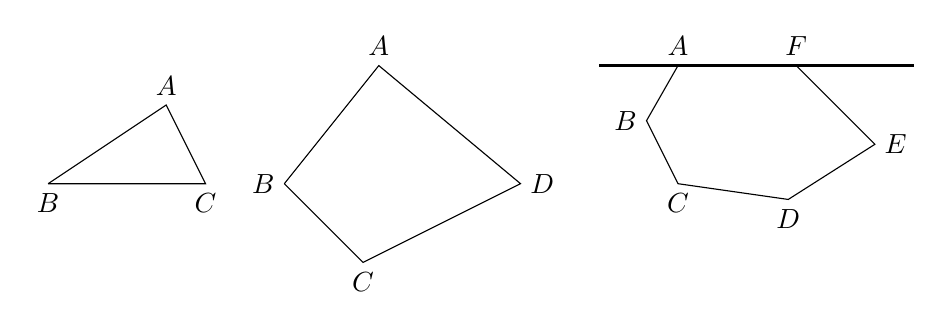
\begin{tikzpicture}
\begin{scope}
\draw(0,0)node[below]{$B$}--(2,0)node[below]{$C$}--(1.5,1)node[above]{$A$}--(0,0);
\end{scope}
\begin{scope}[xshift=3cm]
\draw (0,0)node[left]{$B$}--(1,-1)node[below]{$C$}--(3,0)node[right]{$D$}--(1.2,1.5)node[above]{$A$}--(0,0);
\end{scope}
\begin{scope}[xshift=8cm, yshift=1.5cm]
\draw (0,0)node[above]{$A$}--(1.5,0)node[above]{$F$}--(2.5,-1)node[right]{$E$}--(1.4,-1.7)node[below]{$D$}--(0,-1.5)node[below]{$C$}--(-.4,-.7)node[left]{$B$}--(0,0);
\draw[thick](-1,0)--(3,0);
\end{scope}        
    \end{tikzpicture}
    \caption{}
\end{figure}

\begin{figure}[htp]
    \centering
\begin{tikzpicture}
\draw[dashed](-2,0)--(2,0);
\draw (-.5,0)--(0.2,0)--(.3,-1)--(.7,1.8)--(-.5,0);
\end{tikzpicture}
    \caption{}
\end{figure}

\begin{blk}{定义}
两个能够完全叠合的三角形叫做\textbf{全等三角形}。两
个全等三角形完全叠合时,互相叠合的顶点叫做\textbf{对应点},互
相叠合的边叫做\textbf{对应边},互相叠合的角叫做\textbf{对应角}。因此,
\textbf{全等三角形的对应边相等,对应角相等}。
\end{blk}
 
怎样判定两个三角形全等呢?
\begin{enumerate}
\item 有两边和它们的夹角对应相等的两个三角形全
等。(SAS)
\item 有两角和它们的夹边对应相等的两个三角形全
等。(ASA)
\item 有三边对应相等的两个三角形全等。(SSS)
\end{enumerate}

利用三角形的全等,是判断两条线段或两个角相等的一
种基本方法。













































